\documentclass[11pt]{article}

% load some asm stuff -
\usepackage{amssymb}
\usepackage{amsmath}
\usepackage{amsthm}
%\usepackage{palatino,lettrine}
\usepackage{fancyhdr}
\usepackage{epsfig}
\usepackage[round,comma,sort]{natbib}
\usepackage{simplemargins}
\usepackage{setspace}
\usepackage{wrapfig}
\usepackage{hyperref}
%\usepackage{boiboites}
\usepackage[margin=0pt,font=small,labelfont=bf]{caption}
\newcommand{\boldindex}[1]{\textbf{\hyperpage{#1}}}
\usepackage{makeidx}\makeindex
\bibliographystyle{plos2015}

% Set the size
%\textwidth = 6.75 in
%\textheight = 9.75 in
%\oddsidemargin = 0.0 in
%\evensidemargin = 0.0 in
%\topmargin = 0.01 in
%\headheight = 0.0 in
%\headsep = 0.25 in
%\parskip = 0.15in
% \doublespace
\setallmargins{1in}

\newtheorem{example}{Example}[section]
\newtheorem{thm}{Theorem}[section]
\newtheorem{property}{Property}[section]

\theoremstyle{definition}
\newtheorem{defn}[thm]{Definition}

\makeatletter
\renewcommand\subsection{\@startsection
	{subsection}{2}{0mm}
	{-0.05in}
	{-0.5\baselineskip}
	{\normalfont\normalsize\bfseries}}
\renewcommand\subsubsection{\@startsection
	{subsubsection}{2}{0mm}
	{-0.05in}
	{-0.5\baselineskip}
	{\normalfont\normalsize\itshape\bfseries}}
\renewcommand\paragraph{\@startsection
	{paragraph}{2}{0mm}
	{-0.05in}
	{-0.5\baselineskip}
	{\normalfont\normalsize\itshape}}
\makeatother
\linespread{1.1}

\fancypagestyle{proposal}{\fancyhf{}%
	\fancyhead[RO,LE]{\thepage}%
	\fancyhead[LO,RE]{CHEME 132 Module 1 Binomial Models of Equity Prices}%
	\renewcommand\headrulewidth{1pt}}
\pagestyle{proposal}

\usepackage{mdframed}
\definecolor{lgray}{rgb}{0.92,0.92,0.92}
\definecolor{antiquewhite}{rgb}{0.98,0.92,0.84}
\definecolor{lightskyblue}{rgb}{0.93,0.95,0.99}

% defn environment
\mdfdefinestyle{theoremstyle}{% 
    linecolor=black,linewidth=1pt,% 
    frametitlerule=true,% 
    frametitlebackgroundcolor=lgray, 
    innertopmargin=\topskip,} 
\mdtheorem[style=theoremstyle]{definition}{Definition}

% concept environment
\mdfdefinestyle{conceptstyle}{% 
    linecolor=black,linewidth=1pt,% 
    frametitlerule=true,% 
    frametitlebackgroundcolor=lightskyblue, 
    innertopmargin=\topskip,} 
\mdtheorem[style=conceptstyle]{concept}{Concept}
\newcommand{\newterm}[1]{{\it #1}}

% Single space'd bib -
\setlength\bibsep{0pt}

\renewcommand{\rmdefault}{phv}\renewcommand{\sfdefault}{phv}
%\newboxedtheorem[boxcolor=black, background=gray!5,titlebackground=orange!20,titleboxcolor = black]{color_box_example}{Example}{test}

% Change the number format in the ref list -
\renewcommand{\bibnumfmt}[1]{#1.}

% Change Figure to Fig.
\renewcommand{\figurename}{Fig.}
\usepackage{enumitem}
\setlist{noitemsep} % or \setlist{noitemsep} to leave space around whole list

%Joycelyn Chan, Joshua Lequieu, Michael Paull, Chidanand Balaji, Ryan Tasseff
%Our derivation follows closely the earlier development of Fredrickson \citep{Fredrickson:1976fk}.

% Begin ...
\begin{document}

%\begin{titlepage}
{\par\centering\textbf{\Large CHEME 132 Module 1: Lattice Models of Equity Share Price}}
\vspace{0.2in}
{\par \centering \large{Jeffrey D. Varner}}
\vspace{0.05in}
{\par \centering \large{Smith School of Chemical and Biomolecular Engineering}}
{\par \centering \large{Cornell University, Ithaca NY 14853}}
% \vspace{0.1in}
% {\par \centering \small{Copyright \copyright\ Jeffrey Varner 2018. All Rights Reserved.}}\\

%\end{titlepage}
\date{}
\thispagestyle{empty}

\setcounter{page}{1}

% \begin{mdframed}[backgroundcolor=lgray]

% 	\subsection*{Background}
% 	We have discussed idealized reversible power generation and refrigeration cycles, and considered the impact of
% 	process irreversibility. In this lecture module, we will expand on the topic of irreversibility. In particular, we will develop expressions for
% 	the rate of \textit{lost work} caused by irreversibility in terms if the rate of entropy generation and process unit efficiencies.

% 	\vspace{0.1in}
% 	\subsection*{Student outcomes}
% 	At the end of this lecture module, students will be able to:
% 	\begin{itemize}
% 	  \item[O$_1$]{Describe the terms in the entropy balance for an open time dependent and steady-state system}
% 		\item[O$_2$]{Relate the rate of lost work $\dot{W}_{lost}$ to the rate of entropy generation $\dot{S}_{G}$ in a steady-state system.}
% 		\item[O$_3$]{Relate the efficiency of common equipment, e.g., pumps, compressors turbines etc to the rate of entropy generation $\dot{S}_{G}$ in a steady-state system.}
% 	\end{itemize}

% \end{mdframed}

% \clearpage

\section*{Introduction}
A lattice model discretizes the potential future states of the world into a finite number of options. 
For instance, a binomial lattice model has two future states: \texttt{up} and \texttt{down}, while a ternary lattice model has three: \texttt{up}, \texttt{down}, and \texttt{flat}. 
To make predictions, we must assign values and probabilities to each of these future states and then calculate the expected value and variance of future values. 
Thus, we do not know quantities such as share price exactly because we are projecting into the future. Instead, we have only a probabilistic model of the possible future values. 
We'll begin with the simplest possible lattice model, a binomial lattice (Fig. \ref{fig:binomial-lattice-schematic}).
\begin{figure}[h]
    \centering
    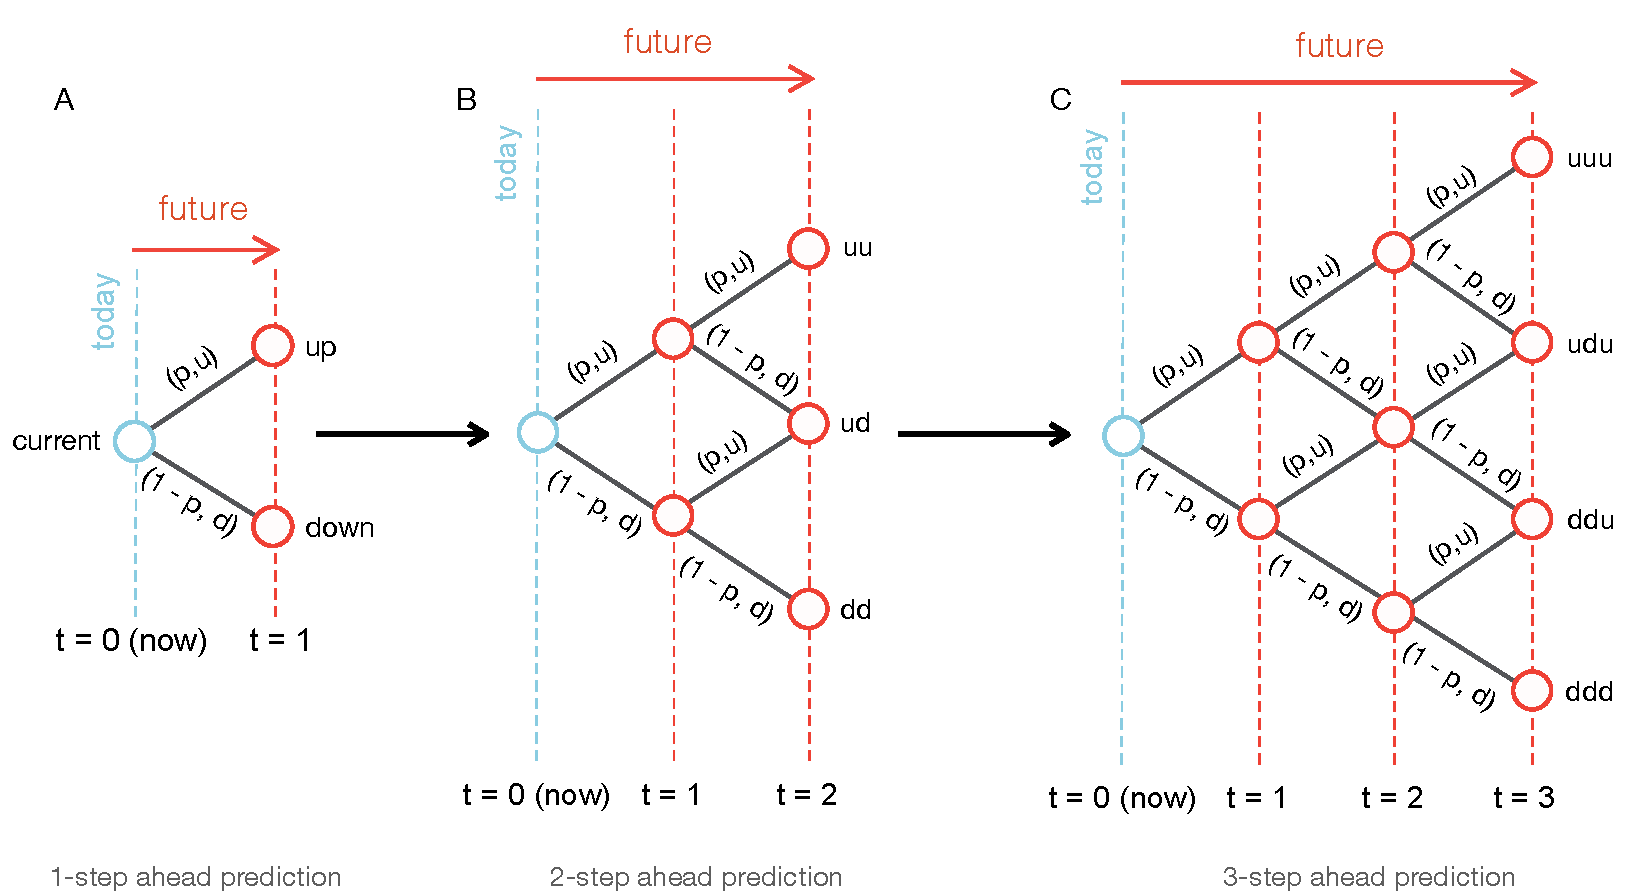
\includegraphics[width=0.85\textwidth]{./figs/Fig-Binomial-LatticeModels-Schematic.pdf}
    \caption{Binomial lattice model schematic. 
	At each node, the share price can either go \texttt{up} by a factor of $u$ or \texttt{down} by a factor of $d$. 
	The probability of going \texttt{up} is $p$ and the probability of going \texttt{down} is $1-p$. 
	\textbf{A}: Single time-step lookahead.
	\textbf{B}: Two time-step lookahead.
	\textbf{C}: Three time-step lookahead.
	At level of the tree $l$, the potential share price can take on $l+1$ values.
	}\label{fig:binomial-lattice-schematic}
\end{figure}

Let's start with a single time-step lookahead, where we have two possible future states (Fig. \ref{fig:binomial-lattice-schematic}A).
Let the initial share price at time \texttt{0} be $S_{\circ}$ and the share price at future time \texttt{1} be $S_{1}$.
During the transition from time \texttt{0}$\rightarrow$\texttt{1} the world transitions from the current state, to one of two possible future states: \texttt{up} or \texttt{down}.
We move to the \texttt{up} state with probability $p$ or the \texttt{down} state with probability $(1-p)$.
Thus, at the time \texttt{1}, the share price $S_{1}$ can take on one of two possible values: $S^{u} = u\cdot{S_{\circ}}$ if the world moves 
to the \texttt{up} state, or $S^{d} = d\cdot{S_{\circ}}$ if the world moves to the \texttt{down} state. 
As we move to the future, we can continue to build out the lattice model by adding additional time-steps, 
for example consider a two-step ahead prediction (Fig. \ref{fig:binomial-lattice-schematic}B). 
At time \texttt{2}, the share price can take on one of three possible values: $S^{uu} = u^{2}\cdot{S_{\circ}}$ if the world moves
to the \texttt{up-up} state, $S^{ud} = ud\cdot{S_{\circ}}$ if the world moves to the \texttt{up-down} state, or $S^{dd} = d^{2}\cdot{S_{\circ}}$ if the world moves to the \texttt{down-down} state.
We can continue to build out the lattice model by adding additional time-steps, for example consider a three-step ahead prediction (Fig. \ref{fig:binomial-lattice-schematic}C).

\section*{Binomial Lattice Model Solution}
Let's consider a binomial lattice model with $n$ time-steps. At each time-step, the share price can either go \texttt{up} by a factor of $u$ or \texttt{down} by a factor of $d$.
Then, at time \texttt{n}, the share price can take on $n+1$ possible values: 
\begin{equation}
	S_{n} = S_{\circ}\times{D_{1}}\times{D_{2}}\times{D_{3}}\times\cdots\times{D_{n}}
\end{equation}
where $D_{i}$ is a random variable that can take on one of two values: $u$ or $d$, 
with probabilities $p$ and $(1-p)$ respectively. 
Thus, at each time-step, the world flips a coin and lands in either the \texttt{up} state with probability $p$ or the \texttt{down} state with probability $(1-p)$.
For a single time-step, we model this random process as a Bernoulli trial, where the probability of success is $p$ and the probability of failure is $(1-p)$.
As the number of time-steps increases we have a series of Bernoulli trials, which is a binomial distribution (Defn: \ref{defn-binomial-distribution}):

\begin{definition}[Binomial Share Price and Probability]\label{defn-binomial-distribution}
	Let $S_{\circ}$ denote the current share price at t = \texttt{0}, $u$ and $d$ denote the \texttt{up} and \texttt{down} factors, 
	and $p$ denote the probability of going \texttt{up}.
	At time $t$, the binomial lattice model predicts the share price $S_{t}$ is given by:
	\begin{equation*}
	S_{t} = S_{\circ}\cdot{u}^{t-k}\cdot{d}^{k}\qquad\text{for}\quad{k=0,1,\dots,t}
	\end{equation*}
	The probability that the share price takes on a partiuclar value at time $t$ is given by:
	\begin{equation*}
	P(S_{t} = S_{\circ}\cdot{u}^{t-k}\cdot{d}^{k}) = \binom{t}{k}\cdot{(1-p)}^{k}\cdot{p}^{t-k}\qquad\text{for}\quad{k=0,1,\dots,t}
	\end{equation*}
	where $\binom{t}{k}$ denotes the binomial coefficient.
\end{definition}

Now that we have a model for the share price and the probability of the share price taking on a particular value, 
we can calculate the expected value and variance of the share price. The expected value of the share price is the 


\section*{Models of $u$, $d$ and $p$}
The \texttt{up} and \texttt{down} factors $u$ and $d$, and the probability $p$ can be defined in various ways.  
For example, we can estimate them from historical data, or we can propose models for their values. 




\clearpage
\printindex

\end{document}
